\documentclass{article}
    \usepackage{amssymb}
    \usepackage[utf8]{inputenc}
    \usepackage[russian]{babel}
    \usepackage[left=2cm,right=2cm,
        top=2cm,bottom=2cm,bindingoffset=0cm]{geometry}
    \usepackage{hyperref}
    \hypersetup{
        colorlinks=true,
        linkcolor=blue,
        filecolor=magenta,      
        urlcolor=cyan,
    }
  \usepackage{graphicx}
  \graphicspath{{pictures/}}
  \DeclareGraphicsExtensions{.pdf,.png,.jpg}

\begin{document}
\begin{center}{\hugeОтчет по курсовой работе за неделю\\}\end{center}
Дата: 15.10.2020\\
Научные руководители: Герасимов С.В., Мещеряков А.В.\\
Студент: Немешаева Алиса\\
Курс: 4\\

\renewcommand{\labelitemi}{$\blacksquare$}
\renewcommand\labelitemii{$\square$}
\begin{enumerate}
    \item На этой неделе продолжалось усовершенствование алгоритма детекции: теперь вместо того, 
        чтобы сканировать каждый патч отдельно и детектировать на нем скопления, алгоритм 
        собирает все патчи в общую карту для большого сегмента неба, чтобы детектировать скопления 
        на нём. Это помогает уменьшить количество false positives, которые появлялись из-за 
        несовершенства старого алгоритма.\\
    \item Были добавлены новые параметры сканирования: теперь для каждого детектированного скопления 
        известны такие свойства, как:
        \begin{itemize}
            \item min\_rad, mean\_rad, max\_rad - минимальный, средний и максимальный радиусы 
                предсказанной маски скопления.\\
            \item min\_pred, max\_pred - минимальный и максимальный prediction index (значение 
                предсказанной маски) скопления.\\
        \end{itemize}
    \item В задаче детекции скоплений важной проблемой является определение массы скопления. 
        Поэтому бывает полезно искать корелляции параметров детектированных скоплений из известных 
        каталогов с массой.\\

    \begin{figure}[h]
        \center{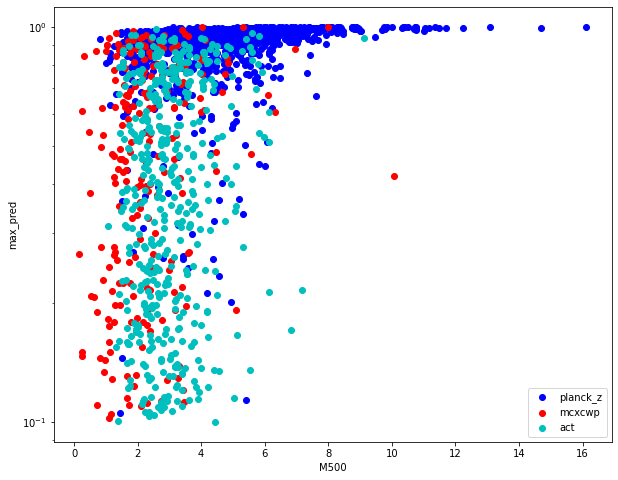
\includegraphics[width=0.6\linewidth]{max_pred_m500}}
        \caption{График соответствия M500 и max\_pred для скоплений true positives.}
    \end{figure}

    \item Кроме того, имеет смысл проверить соответствие параметров z (красное смещение) и M500 
        (масса) для скоплений true positives для того, чтобы иметь возможность формировать каталоги 
        для обучения других моделей - скопления с некоторыми комбинациями параметров скорее всего не 
        получится сегментировать в данных Planck.\\

    \begin{figure}[h]
        \center{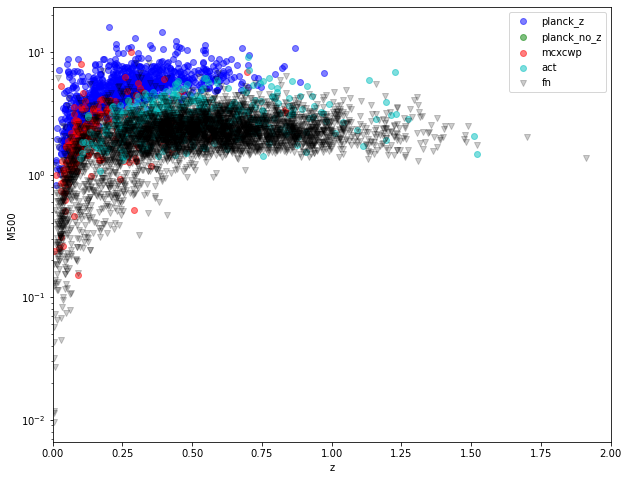
\includegraphics[width=0.6\linewidth]{m500_z}}
        \caption{График соответствия M500 и z для скоплений true positives и false negatives.}
    \end{figure}

\end{enumerate}

Общее количество строк кода за эту неделю: 202\\
\end{document}
